\documentclass[french]{article}
\usepackage[T1]{fontenc}
\usepackage[utf8]{inputenc}
\usepackage{lmodern}
\usepackage[a4paper]{geometry}
\usepackage{babel}
\usepackage{graphicx}

\begin{document}
\title{Nuages de points et modélisation 3D\\
TP 2 : Recalage}
\author{Marius Dufraisse}
\date{}

\maketitle


\paragraph{Question 1.} 
ICP performs well for the bunny only when it is only perturbed, not returned (see Figure \ref{fig:q1-bunny}). For Notre-Dame the results are good too (see Figure \ref{fig:q1-nd12}). The aligned cloud and the reference cloud are not the same as they do not cover the same area. The order used here is important, if the small cloud is used as a reference the ICP will try to align points from the large cloud that don't match points in the small one (see Figure \ref{fig:q1-nd21}). 

\begin{figure}[h]
	\centering
	\begin{minipage}{0.45\linewidth}
		\centering
		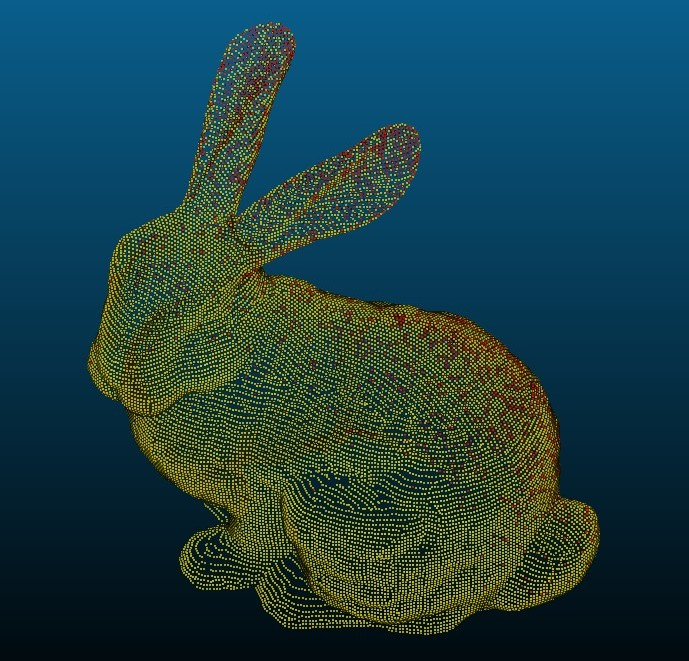
\includegraphics[width=\linewidth]{q1-perturbed.jpg}
	\end{minipage}\hfill
	\begin{minipage}{0.45\linewidth}
		\centering
		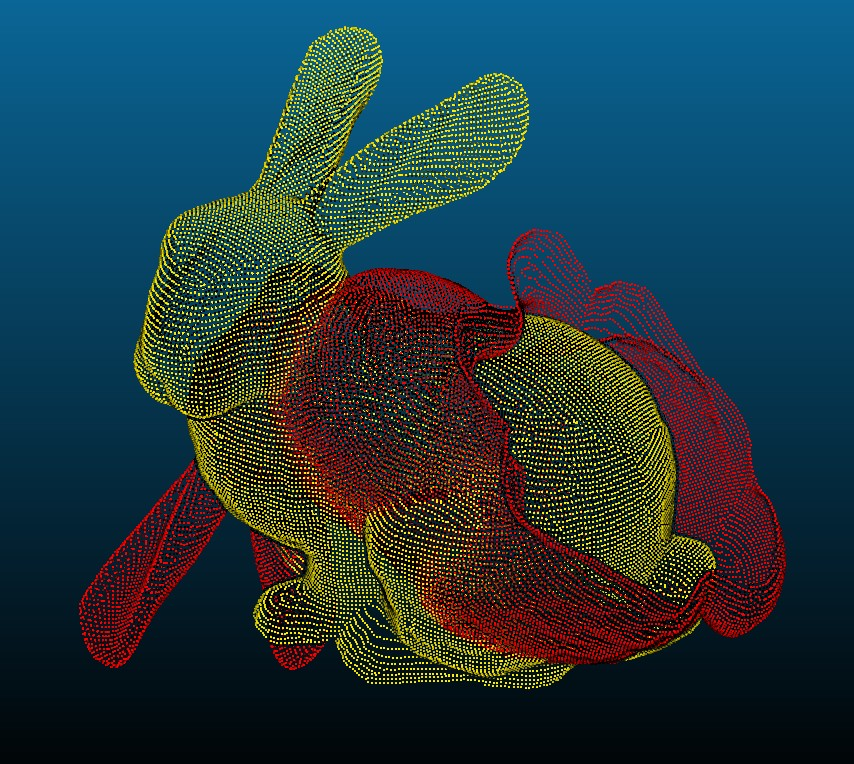
\includegraphics[width=\linewidth]{q1-returned.jpg}
	\end{minipage}
	\caption{Results obtained using CloudCompare implementation of ICP. On the left, the data to align was only slightly perturbed; on the right it was returned.}
	\label{fig:q1-bunny}
\end{figure}

\begin{figure}[h]
	\centering
	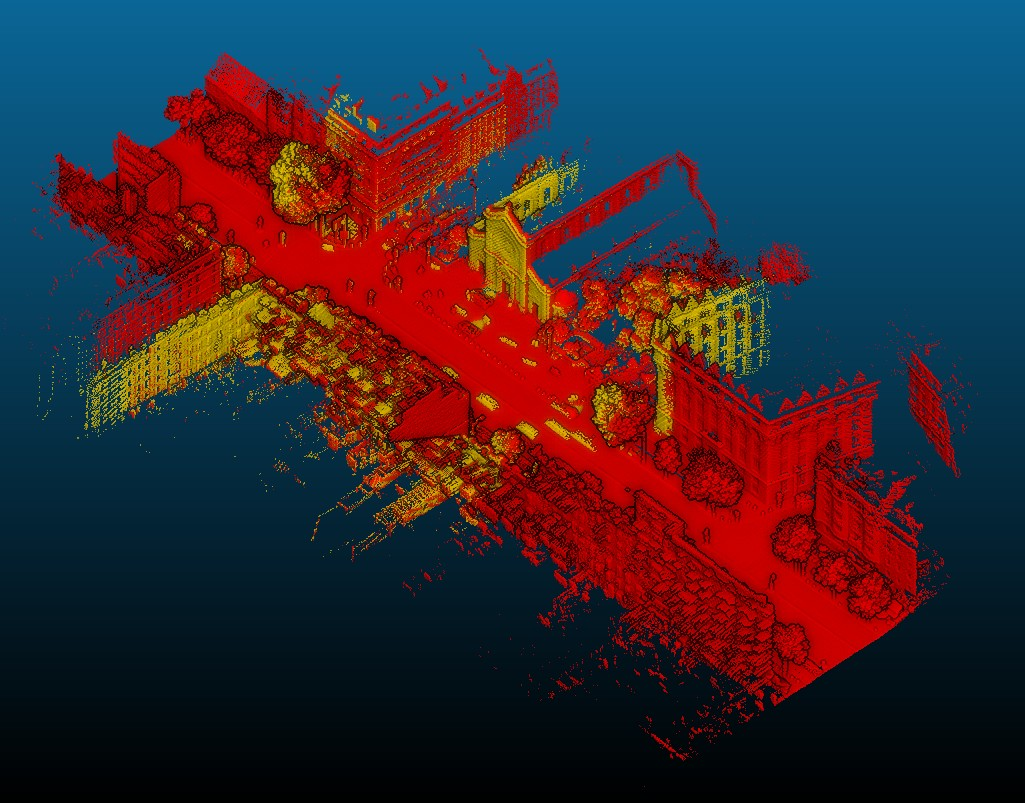
\includegraphics[width=0.6\linewidth]{q1-nd-12.jpg}
	\caption{Results obtained using CloudCompare implementation of ICP on the Notre-Dame point cloud. The larger cloud was used as reference.}
	\label{fig:q1-nd12}
\end{figure}

\begin{figure}[h]
	\centering
	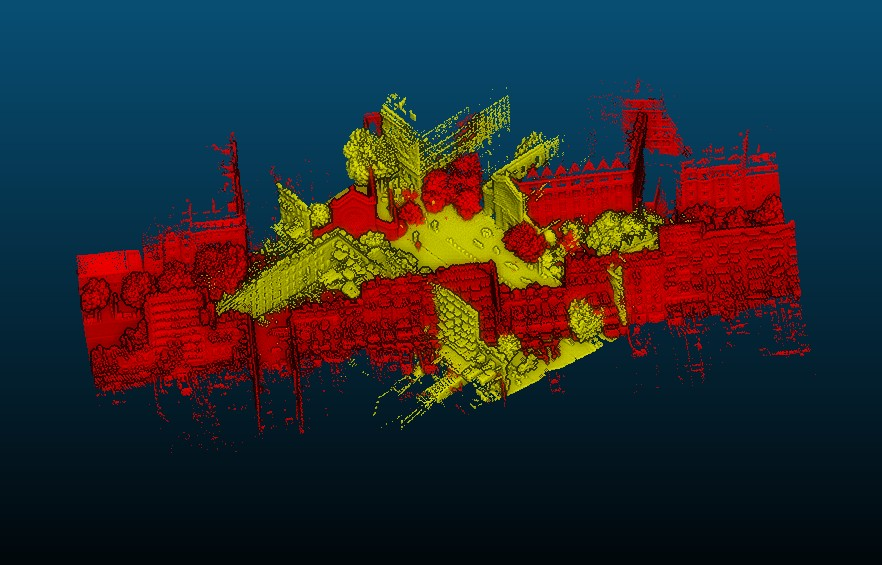
\includegraphics[width=0.6\linewidth]{q1-nd-21.jpg}
	\caption{Results obtained using CloudCompare implementation of ICP on the Notre-Dame point cloud. The smaller cloud was used as reference, as a result the algorithm performed poorly.}
	\label{fig:q1-nd21}
\end{figure}

\end{document}
